\section{Introduction}
This project aims to develop an LLM-based recommender system for Steam games that can interpret natural language queries and generate meaningful recommendations. Unlike traditional systems that rely heavily on exact keyword matching or user-item interaction matrices, this system focuses on understanding the intent behind user queries.

The implemented solution follows a Retrieval-Augmented Generation (RAG) approach, combining structured retrieval with generative modeling to ensure factual and flexible recommendations. This architectural pipeline begins with an initial self-querying step using \texttt{Gemma 3 12B IT}, which serves as both a query optimizer and a robust guardrail for relevance. The retrieval mechanism then employs a hybrid strategy, merging semantic search capabilities with keyword-based search via BM25 to capture both user intent and exact matches. Finally, the system leverages the Gemma model through the Gemini API to refine candidate games and generate grounded, human-like recommendations based on the retrieved context.


\section{Dataset and Preprocessing}
The dataset is stored in a SQLite database (\texttt{steam\_games\_reviews\_25.sqlite}) containing Steam data scraped up to April 2026. It consists of two tables: \texttt{games} and \texttt{reviews}.

The \texttt{games} table includes metadata such as game name, description, genres, tags, price, release date, platform compatibility, and review statistics. The \texttt{reviews} table contains user-generated reviews linked via the game’s application ID, including the review text, language, and a \texttt{weighted\_vote\_score} indicating helpfulness.

To ensure manageable performance, the system indexes up to 5,000 games. Although each game may contain up to 500 English reviews, only the top three reviews per game are used during recommendation. These are selected based on their helpfulness score to ensure that the most informative feedback is prioritised.

Preprocessing was necessary to standardise the data. Tags were extracted from potentially nested structures and reduced to the top eight to prevent excessive noise. Additionally, a combined textual representation was constructed for each game, merging name, genres, tags, and description into a single structured document. Explicit prefixes were added to guide downstream models.

\section{System Architecture}
The system is built as a multi-stage pipeline consisting of query optimisation, hybrid retrieval, re-ranking, and final generation. This design was chosen to maximise both relevance and interpretability.

\begin{figure}[!t]
    \centering
    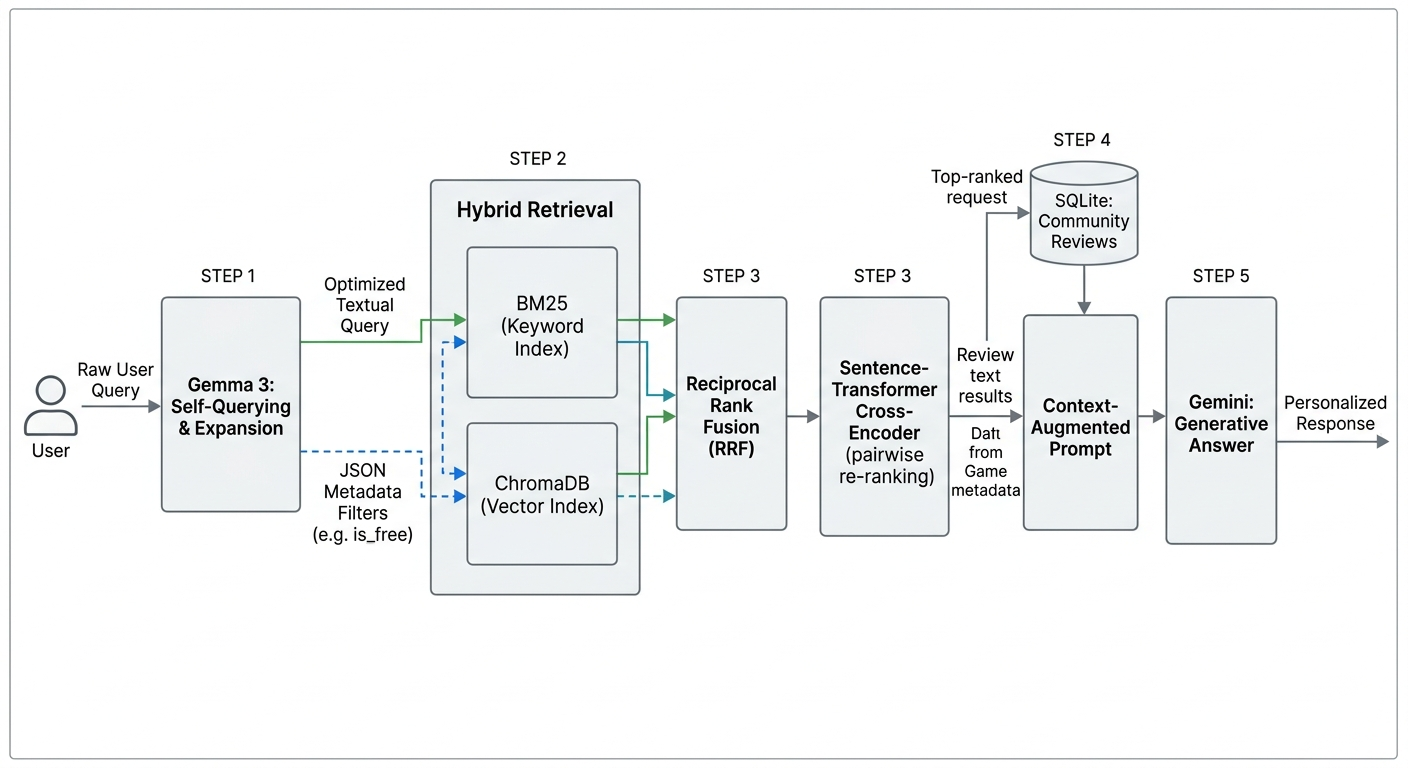
\includegraphics[width=\textwidth]{figures/3_1.png}
    \caption{System Architecture of the RAG-based Steam Recommender System.}
    \label{fig:architecture}
\end{figure}

A key component is the initial self-querying step using \texttt{Gemma 3 12B IT}. The user’s raw query is first rewritten into a more structured and optimised search query. At the same time, the model extracts explicit constraints such as price requirements. For instance, a query requesting ``free games'' is converted into a structured filter that can be applied during retrieval. This step also serves as a guardrail. If the query is unrelated to games, the system returns a \texttt{NOT\_RELEVANT} signal and bypasses the recommendation pipeline entirely.

The backend is implemented in Flask, with indexing performed in a background thread. Additionally, Server-Sent Events (SSE) are used to stream intermediate pipeline information to the frontend, improving transparency and debuggability.

\section{Retrieval, Ranking and Embedding Strategy}
The retrieval stage combines semantic and keyword-based methods. Semantic search is implemented using ChromaDB, which stores vector embeddings of game documents. Keyword search is performed using BM25, which captures exact term matches.

Each method retrieves 30 candidates, which are then merged using Reciprocal Rank Fusion. This approach ensures that both semantic similarity and exact keyword relevance contribute to the final candidate set. Filters extracted during the self-querying stage are applied at this point.

An important design decision concerns the embedding model. Initially, the system was intended to use Google’s Gemini embedding model (\texttt{gemini-embedding-2}) to achieve higher semantic quality. However, during implementation, this approach proved impractical due to strict rate limits in the free API tier. Embedding thousands of games resulted in frequent failures and long runtimes.

As a result, the system was adapted to use the local Sentence Transformers model \texttt{all-MiniLM-L6-v2}. While smaller, this model runs entirely locally and enables fast, stable indexing. Embeddings are stored persistently in ChromaDB with cosine similarity, and batch insertion is used to improve robustness.

After retrieval, candidates are re-ranked using a cross-encoder model (\texttt{ms-marco-MiniLM-L-6-v2}). This model evaluates query–game pairs directly, producing more accurate relevance scores than embedding-based methods alone. The top five results are selected for generation, with an additional heuristic to exclude games explicitly mentioned in the query.

\section{Generation and Use of Reviews}
The final recommendation is generated using the Gemma model via the Gemini API. The prompt includes detailed information for each selected game, such as ranking position, price, release date, tags, review statistics, and a short description.

A crucial component of this stage is the integration of player reviews. For each candidate game, the system performs a real-time SQLite query to retrieve the most relevant reviews:

\begin{lstlisting}[language=SQL, caption=SQL query for fetching top helpful reviews.]
SELECT review FROM reviews 
WHERE appid = ? AND language = 'english' 
ORDER BY weighted_vote_score DESC 
LIMIT 3;
\end{lstlisting}

Rather than performing an additional semantic search over the review corpus, which would introduce significant computational overhead, the system relies on Steam’s built-in community ranking mechanism. Reviews are selected strictly based on their \texttt{weighted\_vote\_score}, which reflects how many users found a review helpful, adjusted through Steam’s internal weighting. By filtering for English-language reviews and selecting only the top-ranked entries, the system effectively uses community consensus as a quality signal.

The impact on recommendation quality is significant. The LLM is explicitly instructed to reference these reviews when generating its response, forcing it to justify recommendations using real player feedback. This enables the system to capture nuances---such as difficulty level, social aspects, or recurring criticisms---that are often absent from developer-written descriptions. Consequently, the generated recommendations are more grounded, balanced, and trustworthy.

\section{Evaluation, Challenges and Future Work}
The system was evaluated through manual testing across a variety of query types, including genre-specific requests, constraint-based queries, and irrelevant inputs. The integration of review data was particularly effective in improving realism.

However, the system introduces noticeable latency due to its multi-stage design. Each query involves multiple steps, including two LLM calls and cross-encoder inference, which increases response time.

Additional challenges included handling inconsistent LLM outputs (such as JSON formatting issues) and ensuring compatibility between metadata and database queries. The dataset size is also limited, which restricts the system’s ability to recommend very niche titles.

\section{Conclusion}
This project demonstrates how LLMs can be effectively integrated into recommender systems using a Retrieval-Augmented Generation framework. By combining hybrid retrieval, cross-encoder re-ranking, and grounded generation, the system is able to produce accurate and context-aware recommendations.

A key insight is that combining semantic and keyword-based retrieval leads to more robust results than relying on a single method. Additionally, incorporating player reviews significantly improves the credibility of the recommendations.

\section{Running the Project}
To ensure that the project can be evaluated without friction, the system has been designed for straightforward setup and execution. The only requirement is a machine running Python 3.10 or higher. As mentioned in the introduction of this report, the complete source code for this system is provided as a supplementary file in the submission and is also publicly available on GitHub for version-controlled auditing.

Dependencies can be installed using \texttt{uv}, which is recommended for speed and reliability:

\begin{lstlisting}[language=bash]
cd raglooker
uv sync
\end{lstlisting}

Alternatively, the required packages can be installed with \texttt{pip}:

\begin{lstlisting}[language=bash]
pip install flask ollama rank-bm25 chromadb sentence-transformers google-genai python-dotenv matplotlib scikit-learn numpy
\end{lstlisting}

The application can then be launched with:

\begin{lstlisting}[language=bash]
uv run app.py
\end{lstlisting}

On first startup, a background daemon thread initialises both the ChromaDB vector database and the BM25 index. The application can then be accessed via the local address shown in the terminal (typically \texttt{http://127.0.0.1:5000}).

\section{Implementation Details}
For a deeper technical dive into the core algorithms described in this chapter, including the self-querying expansion logic, the hybrid Reciprocal Rank Fusion retrieval, and the cross-encoder re-ranking implementation, please refer to the code snippets provided in \textbf{Appendix A}.
